%% This is an example first chapter.  You should put chapter/appendix that you
%% write into a separate file, and add a line \include{yourfilename} to
%% main.tex, where `yourfilename.tex' is the name of the chapter/appendix file.
%% You can process specific files by typing their names in at the 
%% \files=
%% prompt when you run the file main.tex through LaTeX.
\chapter{Introduction}\label{ch1:intro}
The pursuit of energy has shaped the story of mankind from the very beginning. And while the image of ancient humans using fires for warmth, protection, and meal preparation is an archetype of our distant past, modern human needs remain much the same. Lighting to extend day into night, heating and cooling for comfort in our homes, cooking of the food we eat, access to the advanced technologies of our time – these all require energy from one source or another.  Choices abound, from animal and plant-based fuels, to buried resources like various forms of hydrocarbons, to alternatives like solar, wind, hydro, nuclear, and geothermal. How these sources and resources are balanced can shape the growth of societies on the geopolitical stage, as well as grander scale impacts like the future of a habitable Earth and the perseverance and resilience of mankind.

This thesis examines how uncertainty characterization and risk mitigation can increase the role of one source, geothermal, in addressing the ever-growing energy needs in a viable way. This chapter reflects on the extent of those needs and the conditions that may uniquely support an increased focus on geothermal in the near-term. Opportunities and challenges associated with geothermal also lay the foundation for research questions motivating the remainder of this body of work.

\section{Trends in Energy Usage}\label{ch1:trends}
The \acrlong{eia} publishes annual forecasts on U.S. energy generation and consumption in the \acrlong{aeo} report. Based on the 2020 reference case, the \acrshort{aeo} model predicts a 50\% increase in U.S. energy consumption by 2050 (Figure \ref{fig:eia_2021_projections}) and decreasing electricity generation in all sectors except renewables \citep{us_energy_information_administration_annual_2021}. The \acrlong{ieo} shows similar increases in energy demand and renewables consumption, although more traditional sources of energy like coal, natural gas, petroleum, and nuclear also grow to meet the needs of India, China, and other rapidly developing nations \citep{us_energy_information_administration_international_2020}. A deeper look into the 2020 reference case shows solar and wind-based energy generation as the primary drivers in renewables, while geothermal contributions are relatively minor by comparison (Figure \ref{fig:eia_2021_projections}). 
\begin{figure}[htp]
\centering
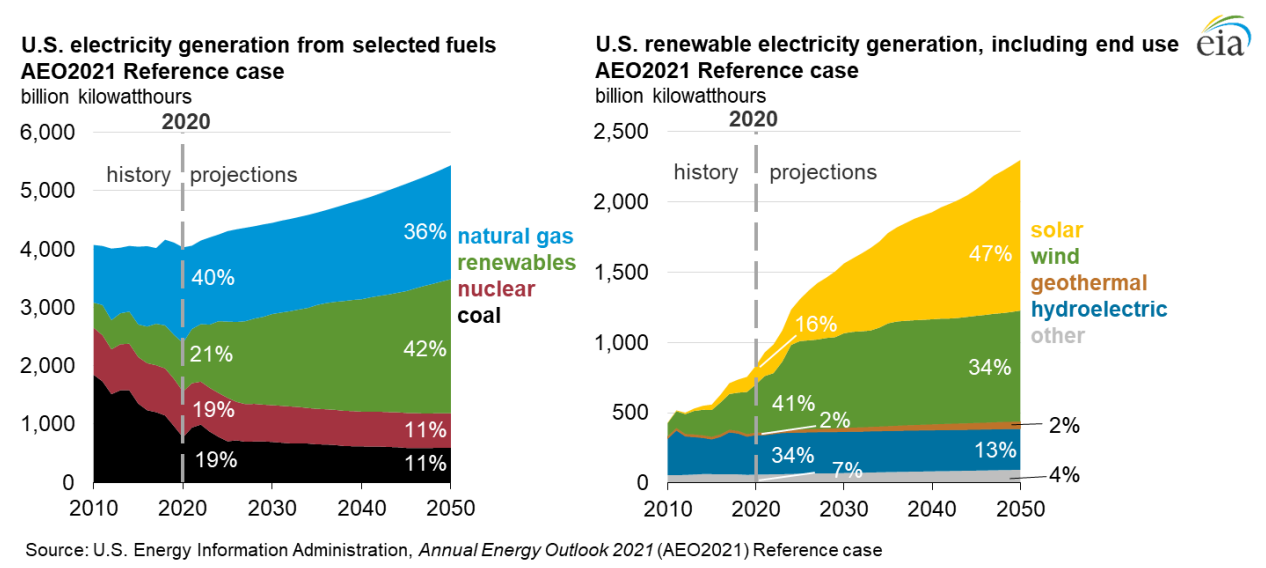
\includegraphics[scale=0.45]{Figure001-EIA_projections}
\caption[U.S. EIA projections based on the AEO2020 reference case]{U.S. EIA projections of (Left) U.S. electricity generation by sector and (Right) individual contributions by renewable type based on the AEO2020 reference case \protect\citep{us_energy_information_administration_annual_2021}}
\label{fig:eia_2021_projections}
\end{figure}

%section~\ref{ch1:sec}.

\section{Upstream Commercial Pressures}\label{ch1:upstream}


\section{Net Zero Ambitions}\label{ch1:netzero}


\section{Geothermal Energy}\label{ch1:geothermal}

\section{Research Questions}\label{ch1:researchqs}


\section{Section sample 2}\label{ch1:sec}

%\footnote{Here is a sample footnote referencing figures~\ref{arm:fig1}
%and~\ref{arm:fig2}.}  


% This is an example of how you would use tgrind to include an example
% of source code; it is commented out in this template since the code
% example file does not exist. To use it, you need to remove the '%' on the
% beginning of the line, and insert your own information in the call.
%
%\tagrind[htbp]{code/pmn.s.tex}{Code sample}{opt:pmn}

%\subsection{Subsection with list}
%\begin{enumerate}
%  \item Item 1.
%  \item Item 2.
%  \item Item 3.
%\end{enumerate}


% This is an example of how you would use tgrind to include an example
% of source code; it is commented out in this template since the code
% example file does not exist.  To use it, you need to remove the '%' on the
% beginning of the line, and insert your own information in the call.
%
%\tgrind[htbp]{code/be.s.tex}{Block Exponent}{opt:be}

%\subsection{Another subsection sample}

%This is done by using some combination of
%\begin{eqnarray*}
%a_i & = & a_j + a_k \\
%a_i & = & 2a_j + a_k \\
%a_i & = & 4a_j + a_k \\
%a_i & = & 8a_j + a_k \\
%a_i & = & a_j - a_k \\
%a_i & = & a_j \ll m \mbox{shift}
%\end{eqnarray*}
%instead of the multiplication.  For example, you could use:
%\begin{eqnarray*}
%r & = & 4s + s\\
%r & = & r + r
%\end{eqnarray*}
%Or by xx:
%\begin{eqnarray*}
%t & = & 2s + s \\
%r & = & 2t + s \\
%r & = & 8r + t
%\end{eqnarray*}
